
%% cross-references, and citations.

\documentclass[11pt]{book}
\usepackage{Wiley-AuthoringTemplate}
\usepackage[sectionbib,authoryear]{natbib}
% for name-date citation comment the below line
%\usepackage[sectionbib,numbers]{natbib}% for numbered citation comment the above line

%%********************************************************************%%
%%       How many levels of section head would you like numbered?     %%
%% 0= no section numbers, 1= section, 2= subsection, 3= subsubsection %%
\setcounter{secnumdepth}{3}
%%********************************************************************%%
%%**********************************************************************%%
%%     How many levels of section head would you like to appear in the  %%
%%				Table of Contents?			%%
%% 0= chapter, 1= section, 2= subsection, 3= subsubsection titles.	%%
\setcounter{tocdepth}{2}
%%**********************************************************************%%

%\includeonly{ch01}
\makeindex
\usepackage{pdfpages}
\usepackage{hyperref}
\newcommand\Emph{\textbf}
\newcommand\p{^{\prime}}
\newcommand\pp{^{\prime\prime}}
\newcommand{\lapl}[1]{\mathscr{L}\{#1\}}
\newcommand{\X}{\mathbb{X}}
\newcommand{\dX}{\dot{\mathbb{X}}}
\newcommand{\fX}{\bar{\text{\b{X}}}}
\newcommand{\ux}{u_x}
\newcommand{\uy}{u_y}
\newcommand{\uxx}{u_{xx}}
\newcommand{\uxy}{u_{xy}}
\newcommand{\uyy}{u_{yy}}
\newcommand{\ut}{u_{t}}
\newcommand{\utt}{u_{tt}}
\newcommand{\second}{2^{\text{nd}}}
\newcommand{\deriv}[2]{\frac{\diff#1}{\diff#2}}
\newcommand{\deriva}[1]{\frac{\diff}{\diff#1}}
\newcommand{\dakuohao}[2]{\left\{\begin{gathered}#1\\#2\end{gathered}\right.}
\newcommand{\dakuohaotri}[3]{\left\{\begin{gathered}#1\\#2\\#3\end{gathered}\right.}
%\includeonly{week10/Wednesday}

\begin{document}

\frontmatter


\booktitle{Partial differential equations}

\subtitle{MAT4022 Notebook}

\AuAff{Prof. Weiming Ni\\ The Chinese University of Hongkong, Shenzhen}


\halftitlepage
\titlepage



\tableofcontents


\acknowledgments
These lecture notes arose from the course ``Partial Differential Equations'' - MAT4022 in fall semester, 2019 taught by Prof.~Ni. Some material is cited from {\it Partial Differential Equations} $4^{th}$ edition by F.John. \\
These notes are copylefted, and may be freely used for noncommercial educational purposes. I will appreciate any and all feedback directed to the e-mail address, 117010345@link.cuhk.edu.cn.
\authorinitials{Xinhao}


\mainmatter
\setcounter{page}{1}


\chapter{Week4}

\section{Tuesday}\index{Tuesday_lecture}
\subsection{Inhomogeneous Wave Equation}
\[\dakuohaotri{u_{tt}-c^2u_{xx}=f(x,t)\qquad x\in[o,L], ~t\geq0}{u(x,0)=\varphi(x), u_t(x,0)=\psi(x), ~x\in[0,L]}{u(0,t)=h(t), ~u(L,t)=k(t)}
\]
Assume $h(0)=k(0)=0$.Write 
 \[u(x,t)=\sum_{n=1}^\infty u_n(t)\sin\frac{n\pi x}{L},~u_n(t)=\frac{2}{L}\int_0^L u(x,t)\sin\frac{n\pi x}{L}\diff x\] 
\[\quad f(x,t)=\sum_{n=1}^\infty f_n(t)\sin\frac{n\pi x}{L},~f_n(t)=\frac{2}{L}\int_0^L f(x,t)\sin\frac{n\pi x}{L}\diff x\]
\[u_{tt}(x,t)=\sum_{n=1}^\infty V_n(t)\sin \frac{n\pi x}{L},\quad  V_n(t)=\frac{2}{L}\int_0^L u_{tt}(x,t)\sin \frac{n\pi x}{L}\diff x=\frac{\diff^2u_n}{\diff t}
\]
\[u_{xx}(x,t)=\sum_{n=1}^\infty w_n(t)\sin\frac{n\pi x}{L},\quad w_n(t)=\frac{2}{L}\int_0^L u_{xx}(x,t)\sin \frac{n\pi x}{L}\diff x
\]
\[\begin{aligned}w_n(t)&=\frac{2}{L}\int_0^L \uxx(x,t)\sin\frac{n\pi x}{L}\diff x\\
&=\frac{2}{L}[\ux\sin\frac{n\pi x}{L}|_0^L-\frac{n\pi}{L}\int_0^L\ux\cos \frac{n\pi x}{L}\diff x]\\
&=-\frac{2n\pi}{L^2}[n\cos\frac{n\pi x}{L}|_0^L+\frac{n\pi}{L}\int_0^Lu\sin\frac{n\pi x}{L}\diff x]\\
&=-\frac{2n\pi}{L^2}[u(L,t)(-1)^n-u(0,t)+\frac{n\pi}{L}\int_0^Lu\sin\frac{n\pi x}{L}\diff x]\\
&=-\frac{2n\pi}{L^2}[(-1)^nk(t)-h(t)+\frac{n\pi}{2}u_n(t)]\\
&=\frac{2n\pi}{L^2}[h(t)-(-1)^nk(t)]-(\frac{n\pi}{L})^2u_n(t)
\end{aligned}
\]
\[v_n(t)-c^2w_n(t)=\frac{2}{L}\int_0^L(u_{tt}-c^2\uxx)\sin\frac{n\pi x}{L}\diff x=\frac{2}{L}\int_0^Lf(x,t)\sin\frac{n\pi x}{L}\diff x=f_n(t)
\]
\[\frac{\diff^2u_n}{\diff t^2}+c^2\lambda_nu_n(t)-\frac{2n\pi}{L^2}[h(t)-(-1)^nk(t)]c^2=f_n(t),~n\geq1
\]
Solve this ODE of $u_n$, we get the solution.\\
%\[\dakuohao{u_tt-c^2\uxx=f(x,t)}{u(0,t)=u(L,t)=0}
%\]
\[\dakuohao{u_{tt}-c^2\uxx=f(x,t)}{u(0,t=u(L,t)=0}
\]
To solve
\[\dakuohao{U_{tt}-c^2U_{xx}=g(x,t)}{U(0,L)=h(t), U(L,t)=k(t)}
\]
Set $\rho(x,t)=\frac{(L-x)}{L}h(t)+\frac{x}{L}k(t)~\Rightarrow~ \rho(0,t)=h(t),~\rho(L,t)=k(t)$
\[u(x,t)=U(x,t)-\rho(x,t)
\]
\[u_{tt}-c^2\uxx=U_{tt}-c^2U_{xx}-\rho_{tt}+c^2\rho_{xx}=g(x,t)-\frac{L-x}{L}h_{tt}-\frac{x}{L}k_{tt}=f(x,t)
\]
Set $U(x,t)=u(x,t)+\frac{L-x}{L}h(t)+\frac{x}{L}k(t)$.


%%%%%%%%%%%%%%%%%%
To solve the given inhomogeneous problem
\[\dakuohao{U_{tt}-c^2U_{xx}=g(x,t)}{U(0,L)=h(t), U(L,t)=k(t)}
\]
Set $f(x,t)=g(x,t)-\frac{L-x}{L}h_{tt}(t)-\frac{x}{L}k_{tt}(t)$ and we know the solution for $\dakuohao{u_tt-c^\uxx=f(x,t)}{u(0,t)=0,~u(L,t)=0}$ Then $U(x,t)=u(x,t)+\frac{L-x}{L}h(t)+\frac{x}{L}k(t)$ solves.
%%%%%%%%%%%%
Solve $\dakuohao{v_{tt}-c^2v_{xx}=0}{v(x,0)=\varphi(x), v_t(x,0)=\psi(x)}\Rightarrow U+v$\\

\[\dakuohaotri{u_{tt}-c^2\uxx=f(x,t)\quad x\in\mathbb{R},t\geq0}{u(x,0)=\varphi(x)}{u_r(x,0)=\psi(x)}
\]
\[u(x,t)=\frac{1}{2}(\varphi(x+ct)+\varphi(x-ct))+\frac{1}{2c}\int_{x-ct}^{x+ct}\psi(y)\diff y+\frac{1}{2c}\int\int_Df(y,s)\diff y\diff s
\]
Duhamel's Principle
\[\dakuohaotri{\frac{\diff^2v}{\diff t^2}+A^2v=f(t)}{v(0)=a}{v\p(0)=b}
\]
Let $S(t)=\frac{1}{A}\sin At~\Rightarrow ~v(t)=S\p(t)a+S(t)b+\int_0^tS(t-s)f(s)\diff s$\\
Pluge $S$ in the system of equations. We get the solution. (Remind what we do in ODE with variation of parameter. This two method is the same in essence. In addition, what we do in PDE is similiar.)
















\chapter{week3}

\section{Thursday}\index{Thursday_lecture}
\subsection{Fourier Series}
On $[-\pi,\pi]$ want to approximate $f(x)$ by $a_0+a_1\cos x+b_1\sin x+a_2\cos 2x+b_2\sin 2x+\dots+a_k\cos kx+b_k \sin kx+\dots$.\\
Want to show $\{1,\cos x,\sin x,\cos 2x,\sin 2x,\dots,\cos kx,\sin kx,\dots\}$ is a family of orthoganol functions s.t. they for a basis of continuous function space.\\
Inner product:
\[<f,g>=\int_{-\pi}^{\pi}f(x)g(x)\diff x
\]
The following is aim to show it is a orthoganol family.\\
\[<1,\cos kx>=\int_{-\pi}^\pi 1\cdot\cos kx \diff x=\frac{1}{k}\sin kx|_{-\pi}^\pi=0
\]
\[<1,\sin lx>=\int_{-\pi}^\pi 1\cdot \sin lx\diff x=-\frac{1}{L}\cos lx|_{-\pi}^\pi=0
\]
\[\begin{aligned}<\cos kx,\cos lx>&=\int_{-\pi}^\pi]\cos kx\cos lx\diff x\\
&=\frac{1}{2}\int_{-\pi}^\pi[\cos(k+l)x+\cos(k-l)x]\diff x\\
&=\frac{1}{2}\int_{-\pi}^\pi \cos(k-l)x\diff x\\
&=\begin{cases}0 \text{ if } k\neq l\\\pi \text{ if } k=l\neq0\end{cases}
\end{aligned}
\]
Next we are going to find all their coefficient.\\
Assume $f(x)=a_0+\sum_{k=1}^\infty(a_k\cos kx+b_k\sin kx)$.
\[<f,1>=\int_{-\pi}^\pi f(x)\diff x\Rightarrow a_0=\frac{1}{2\pi}\int_{-\pi}^\pi f(x)\diff x
\]
\[<a_0+\sum_{k=1}^{\infty}(a_k\cos kx+b_k\sin kx),1>=<a_0,1>+\sum_{k=1}^{\infty}<a_k\cos kx+b_k\sin kx,1>=<a_0,1>=2\pi a_0
\]
\[<f,\cos x>=<a_0,\cos x>+\sum_{k=1}^\infty[<a_k\cos kx,\cos x>+<b_k\sin kx,\cos x>]=<a_1\cos x,\cos x>=a_1\pi
\]
\[a_1=\frac{1}{\pi}\int_{-\pi}^\pi f(x)\cos x\diff x
\]
\[b_1=\frac{1}{\pi}\int_{-\pi}^\pi f(x)\sin x\diff x
\]
\[a_k=\frac{1}{\pi}\int_{-\pi}^\pi f(x)\cos kx\diff x
\]
$a_0+\sum_{k=1}^N(a_k\cos kx+b_k\sin kx)\rightarrow f(x)$ for as $N\rightarrow \infty$  $\{1,\cos x,\sin x,\cos 2x,\sin 2x,\dots,\cos kx,\sin kx,\dots\}$ form a complete basis for function space.\\
\[*\dakuohaotri{X\pp+\lambda X=0  \text{ in }(a,b)}{a_1X(a)+a_2X\p(a)=0}{\beta_1X(b)+\beta_2X\p(b)=0}
\]
$\alpha_1, \alpha_2, \beta_1, \beta_2$ are constants. $\alpha_1^2+\alpha_2^2>0,  \beta_1^2+\beta_2^2>0$
\begin{theorem}
(1) The eigenvalues of (*) form an increasing sequence $\lambda_1<\lambda_2<\lambda_3<\dots<\lambda_k<\dots\rightarrow \infty $.\\
(2)For each eigenvalue $\lambda_k$ the corresponding eigenspace is 1-dimensional. Denote eigen function by $X_k$.\\
(3) $X_k$ has exactly $k-1$ zeros in $(a,b)$.\\
(4) $\{X_1, X_2, \dots, x_k,\dots\}$ is a family of orthogonal $f(n)$ i.e. $\int_a^b x_kx_l=0$ if $k\neq l$.\\
(5)If $\varphi(x)$ is $C^2[a,b]$ then its eigen function expansion $\sum_{k=1}^\infty \varphi_k X_k$ converges to $\varphi(x)$ uniformly on $[a,b]$ when $\varphi_k=\frac{\int_a^b\varphi(x)X_k(x)\diff x}{\int_a^bX_k^2(x)\diff x}$\\
(6)If $\varphi$ is only square intergrable i.e. if $\int_a^b\varphi^2(x)\diff x<\infty$, then $\int_a^b[\varphi(x)-\sum_{k=1}^N\varphi_kX_k(x)]^2\diff x]\rightarrow 0$ as $N\rightarrow \infty$.


\end{theorem}
(1)$\dakuohao{\alpha_1=1, \alpha_2=0}{\beta_1=1, \beta_2 =0}$ Dirichlet\\
(2)$\dakuohao{\alpha_1=0,\alpha_2=1}{\beta_1=0, \beta_2=1}$ Neumann.\\
The following is going to show when two solutions of $x\pp+\lambda x=0$ are different. $x_k$ is orthorganol to $x_l$.\\
\[\dakuohao{x_k\pp+\lambda_kx_k=0}{x_l\pp+\lambda_lx_l=0}
\]
Multiply $x_l$ and $x_k$ correspondingly to two equations and then take the integral. We have
\[0=\int_a^b(x_k\pp x_l-x_l\pp x_k)+\int_a^b(\lambda_k-\lambda_l)x_kx_l=(x_k\p-x_l\p-x_l\p x_k)|_a^b+\int_a^b(\lambda_k-\lambda_l)x_kx_l
\]
\[=x_k\p(b)x_l(b)-x_l\p(b)x_k(b)-x_k\p(a)x_l(a)+x_l\p(a)x_k(a)+\int_a^b(\lambda_k-\lambda_l)x_kx_l=0
\]
\[\int_a^bx_kx_l=0
\]
Sturm-Liouville
\[\deriva{x}(p(x)\deriv{u}{x})+1(x)u=0
\]







\chapter{week2}

\section{Tuesday}\index{Tuesday_lecture}
\subsection{Quasi-linear Equations}
Review: last week we have learn how to solve the following PDE and get the solution along characteristic curves.
\[\uy+c\ux=0\qquad x\ux+y\uy=u
\]
\begin{figure}[H]
\centering
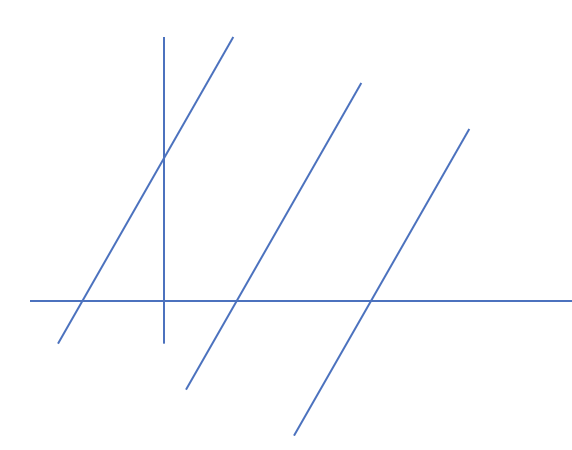
\includegraphics[width=3cm]{week2_tuesday1}
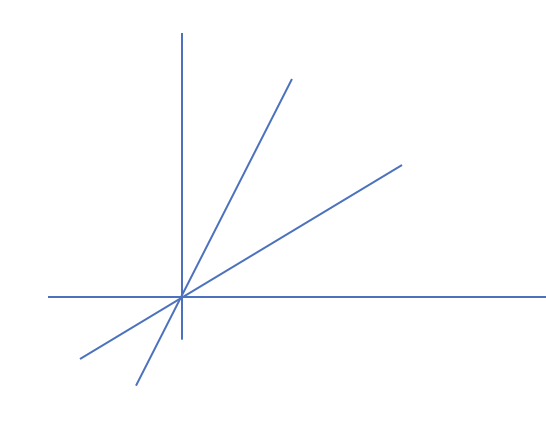
\includegraphics[width=3cm]{week2_tuesday2}
\end{figure}
\[a(x,y,u)\ux+b(x,y,u)\uy=c(x,y,u)
\]
This is what we called quasi-linear equation. At this time, I have to quote our textbook p9 since I cannot explain what professor said better than it does.
\begin{figure}[H]
\centering
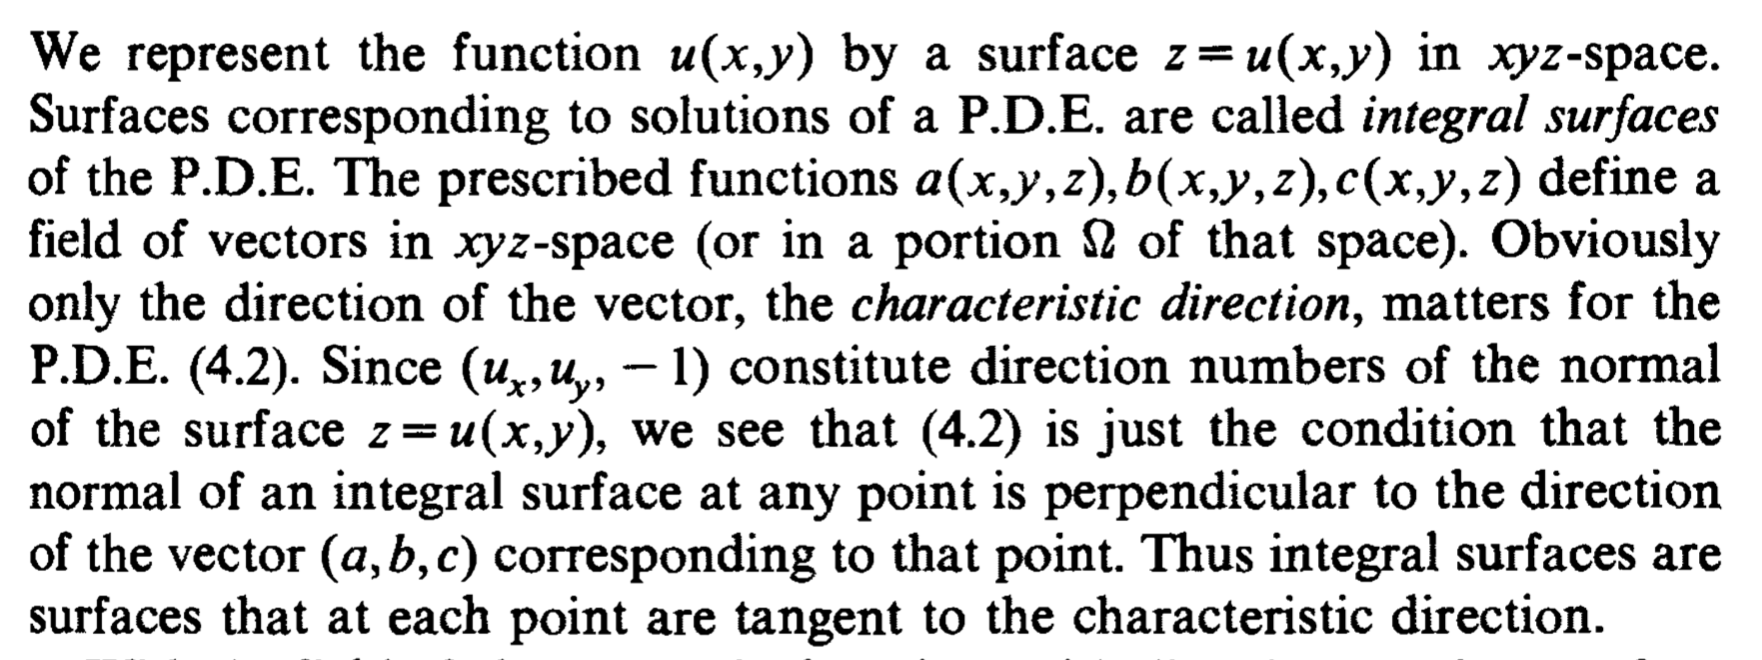
\includegraphics[width=15cm]{week2_tuesday3}
\end{figure}
\begin{figure}[H]
\centering
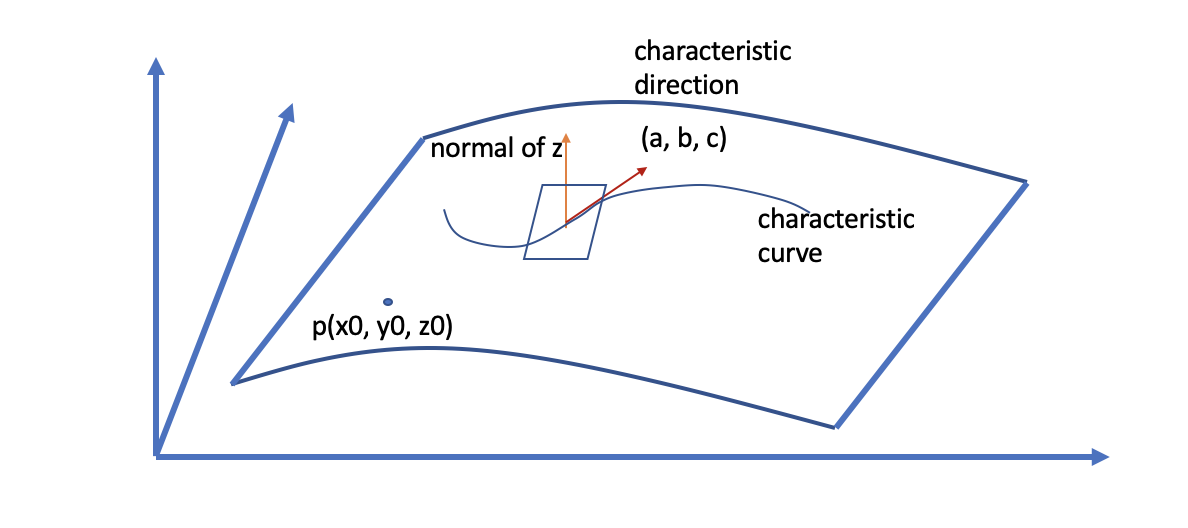
\includegraphics[width=15cm]{week2_tuesday4}
\end{figure}
Next we are going to show that the integral surface, that is the solution $u$ we want, is the union of characteristic curves.
\begin{theorem}
If a characteristic curve $\mathscr{C}$ has one point on a integral surface $z=u(x,y)$ then $\mathscr{C}$ lies entirely on the surface.

\end{theorem}
\begin{proof}
\[z_0=u(x_0,y_0)
\]
\[\left\{\begin{gathered}\deriv{x}{t}=a(x(t),y(t),u(x_0,y_0))\\\deriv{y}{t}=b(x(t),y(t),u(x_0,y_0))\\x(0)=x_0\\y(0)=y_0\end{gathered}\right.
\]
This is a system of odes, there is a solution ($x(t),y(t)$) when $t$ is around 0.\\
This gives us a curve $(x(t),y(t),u(x(t),y(t)))$ lies on the integral surface.\\
Claim: It's a characteristic curve.
\[z(t)=u(x(t),y(t))
\]
\[\deriv{z}{t}=\ux\deriv{x}{t}+\uy\deriv{y}{t}=a\ux+b\uy=c
\]



\end{proof}
\subsection{Cauchy Problem}
``We now have a simple description for the general solution $u$ of the quasilinear equation. To have a better insight into the structure of the manifold of solutions it is desirable to have a definite method of generating solutions in terms of a prescribed set $F$ of functions, called ``data''.''(John, 1982, p.11)\\
``Finding the function $u(x,y)$ for given data $x=f(s)$, $y=g(s)$, $u=h(s)$ constitutes the \text{\it Cauchy problem} for quasi-linear equation.'' (John, 1982, p.9)\\ The following $\varphi, \psi, \rho$ are $f, g, h$ correspondingly.\\
To solve the Cauchy problem, it suffices to require that $(\psi\p,\varphi\p)\&(a,b)$ are linearly independent.\\The
\[\left\{\begin{gathered}\deriv{\bar{X}}{t}=a(\bar{X},\bar{Y},Z)\\\deriv{\bar{Y}}{t}=b(\bar{X},\bar{Y},Z)\\\deriv{\bar{z}}{t}=c(\bar{X},\bar{Y},Z)\\\bar{X}(s,0)=\varphi(s)\\\bar{Y}(s,0)=\psi(s)\\\bar{Z}(s,0)=\rho(s)\end{gathered}\right.
\]
Existence and uniqueness theorem for ODE.\\
$\Rightarrow$ For every $s$, $\exists$ one solution $(\bar{X}(s,t),\bar{Y}(s,t),z(s,t))$. In order to make $u(x,y)=z(s(x,y),t(x,y))$ is the case. We need implicit function theorem which makes us able to write $s, t$ as a function of $(x,y)$
\[\begin{vmatrix}\frac{\partial{\bar{X}}}{\partial{s}}&\frac{\partial{\bar{X}}}{\partial{t}}\\\frac{\partial{\bar{Y}}}{\partial{s}}&\frac{\partial{\bar{Y}}}{\partial{t}}\end{vmatrix}=\begin{vmatrix}\varphi\p&a\\\psi\p&b\end{vmatrix}\neq0
\]
\begin{example}
\[\uy+u\ux=0, \quad u(x,0)=f(x)\]
\[\deriv{x}{t}=z,~\deriv{y}{t}=1,~\deriv{z}{t}=0
\]
$z$ is constant in $t$. $z(s, 0)=f(s)\Rightarrow z(s,t)=f(s)$.
\[\dakuohao{x(s,0)=s~\Rightarrow~x(s,t)=f(s)t+s}{y(s,0)=0~\Rightarrow~y(s,t)=t}\rightarrow ~s=x-f(s)t=x-f(s)y=x-zy
\]
\[z(s,0)=f(s)\Rightarrow z(s,t)=f(s)=f(x-zy)
\]
\[u(x,y)=f(x-uy)
\]
Characteristic curve
\[f(s_2)>f(s_3)
\]
\[\frac{1}{f(s_2)}<\frac{1}{s_3}
\]
Why it is called a ``Shock''?\\The reason is that: for same $(x,y)$ $z$ should be the same. However, from the graph we can see there are two $z$ corresponds to the same point marked by the circle. Therefore, the solution does't exist.
\begin{figure}[H]
\centering
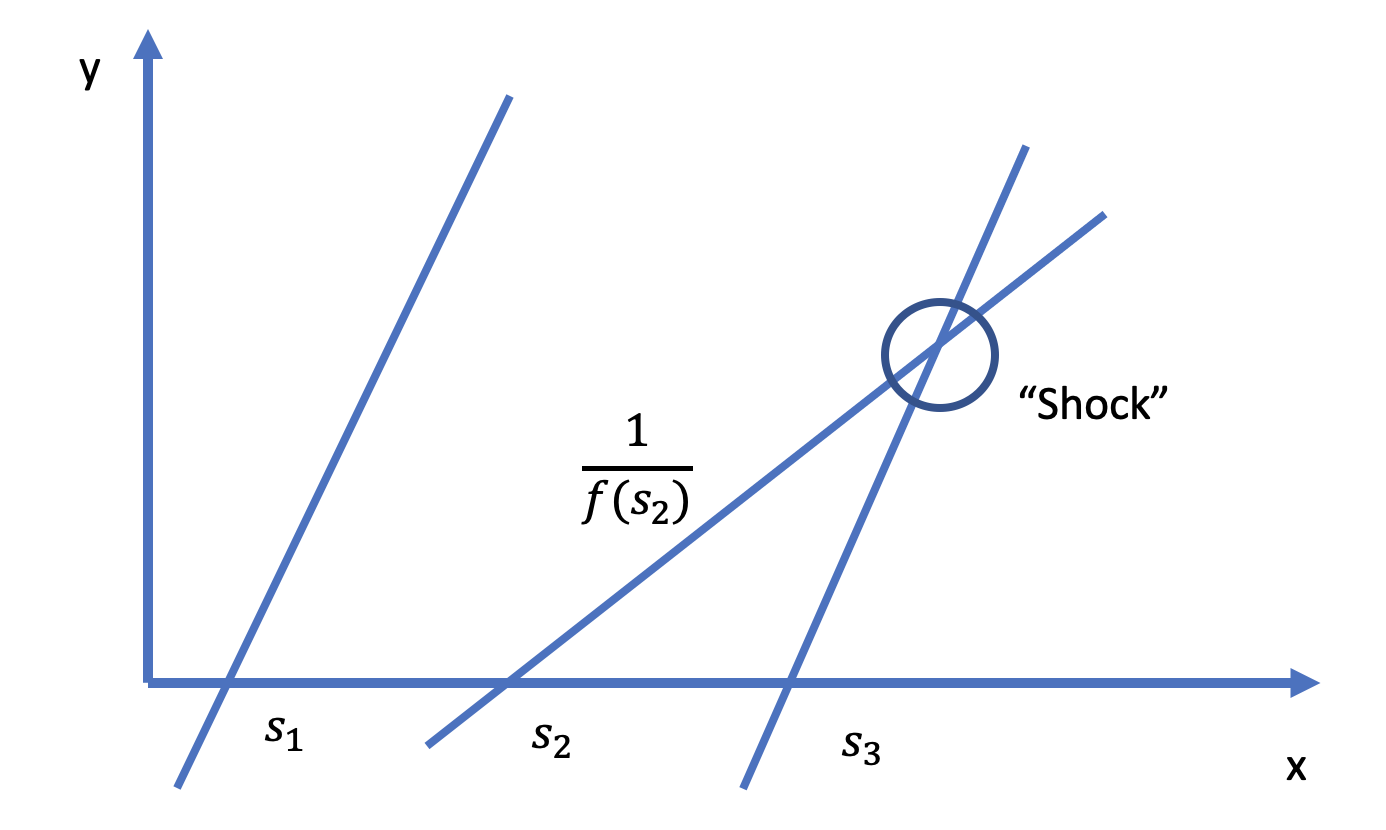
\includegraphics[width=8cm]{week2_tuesday5}
\end{figure}



\end{example}

\section{Thursday}\index{Thursday_lecture}
\subsection{$\second$ order Quasi-linear}
\[a\uxx+2b\uxy+c\uyy=d
\]
$a$, $b$, $c$, $d$ are functions of $(x,y,u,\ux,\uy)$\\
Initial curve $f(s)$, $g(s)$. Initial value $u=h(s),\ux=\varphi(s), \uy=\psi(s)$.\\
\[u(f(s),g(s))=h(s)
\]
\[\ux f\p+\uy g\p=h\p
\]
\[\varphi f\p+\psi g\p=h\p
\]
Assume the above equation is satisfied.
\[\ux(f(s),g(s))=\varphi(s)\qquad\uy(f(s),g(s))=\psi(s)
\]
\[\uxx f\p+\uxy g\p=\varphi \p\qquad u_{yx}f\p+\uyy g\p=\psi\p
\]
\[\begin{pmatrix}a&2b&c\\f\p&g\p&0\\0&f\p&g\p\end{pmatrix}\begin{pmatrix}\uxx\\\uxy\\\uyy\end{pmatrix}=\begin{pmatrix}d\\\varphi\p\\\psi\p\end{pmatrix}
\]
\[0=\begin{vmatrix}a&2b&c\\f\p&g\p&0\\0&f\p&g\p\end{vmatrix}=a{g\p}^2-2bf\p g\p+c{f\p}^2
\]
Personal understanding (may not be correct):\\
This is called characteristic curve for when determinant is equal to zero above system will not have a solution. This situation will on happen when the initial curve $(f,g,h)$is tangent to a charateristic curve at every point. Therefore, $a{g\p}^2-2bf\p g\p+c{f\p}^2$.
\[\dakuohao{x=f(s)}{y=g(s)}\quad\dakuohao{\deriv{x}{s}=f\p}{\deriv{y}{s}=g\p}~\Rightarrow~\deriv{y}{x}=\frac{g\p}{f\p}
\]
\[a(\deriv{y}{x})^2-2b\deriv{y}{x}+c=0
\]
\[\deriv{y}{x}=\frac{2b\pm\sqrt{2b^2-4ac}}{2a}
\]
\begin{itemize}
\item $b^2-ac>0$: Hyperbolic
\item $b^2-ac=0$: Parabolic
\item $b^2-ac<0$: Elliptic

\end{itemize}
\begin{example}

\begin{itemize}
\item $\uyy-c^2\uxx=0$ $A=-c^2, B=0, C=1\Rightarrow~B^2-AC=C^2$
\item heat equation $\uy=c^2=\uxx=0$  $A=-C^2, B=0, C=0~\Rightarrow~B^2-AC=0$
\item laplace equation $\uyy+\uxx=0$ $A=1=C, B=0~\Rightarrow~B^2-AC=-1<0$
\end{itemize}
\end{example}

Wave equation
\[\uyy-c^2\uxx=0
\]
\[\deriv{y}{x}=\frac{1}{-c^2}(\pm c)=\mp\frac{1}{c}
\]
\[y=\mp\frac{1}{c}x+\text{const}
\]
\[y\pm\frac{1}{c}x=\text{const}
\]
\[\xi=y+\frac{1}{c}x
\]
\[\eta=y-\frac{1}{c}x
\]
\[v(\xi,\eta)=u(x(\xi,\eta),y(\xi,\eta))
\]
\[u(x,y)=v(\xi(x,y),\eta(x,y))
\]
\[\ux=v_{\xi}\xi_{x}+v_\eta\eta_x=v_{\xi}\frac{1}{c}-v_\eta\frac{1}{c}
\]
\[\uxx=v_{\xi\xi}\frac{1}{c^2}+v_{\xi\eta}(-\frac{1}{c^2})-v_{\eta\xi}\frac{1}{c^2}+v_{\eta\eta}\frac{1}{c^2}
\]
\[\uy=v_\xi\xi_y+v_\eta\eta_y=v_\xi+v_\eta
\]
\[\uyy=v_{\xi\xi}+2v_{\xi\eta}+v_{yy}
\]
\[0=\uyy-c^2\uxx=v_{\xi\xi}+2v_{\xi\eta}+v_{yy}-v_{\xi\xi}+2v_{\xi\eta}-v_{\eta\eta}=4v_{\xi\eta}
\]
\[v_{\eta\xi}=0~\Rightarrow~(v_\xi)_\eta=0~\Rightarrow ~v_\xi=f\p(\xi)
\]
\[v=f(\xi)=\text{const in }\xi
\]
\[v(\xi,\eta)=f(\xi)+g(\eta)=u(x,y)=f(y+\frac{1}{c}x)+g(y-\frac{1}{c}x)
\]
An observation:
\[u(A)+u(C)=f(y_A+\frac{1}{c}x_A)+g(\underline{\red y_A-\frac{1}{c}x_A})+f(y_C\frac{1}{c}x_C)+g(y_C-\frac{1}{c}x_C)
\]
\[u(B)+u(D)=f(y_B+\frac{1}{c}x_B)+g(\underline{\red y_B-\frac{1}{c}x_B})+f(y_D\frac{1}{c}x_D)+g(y_D-\frac{1}{c}x_D)
\]
\begin{figure}[H]
\centering
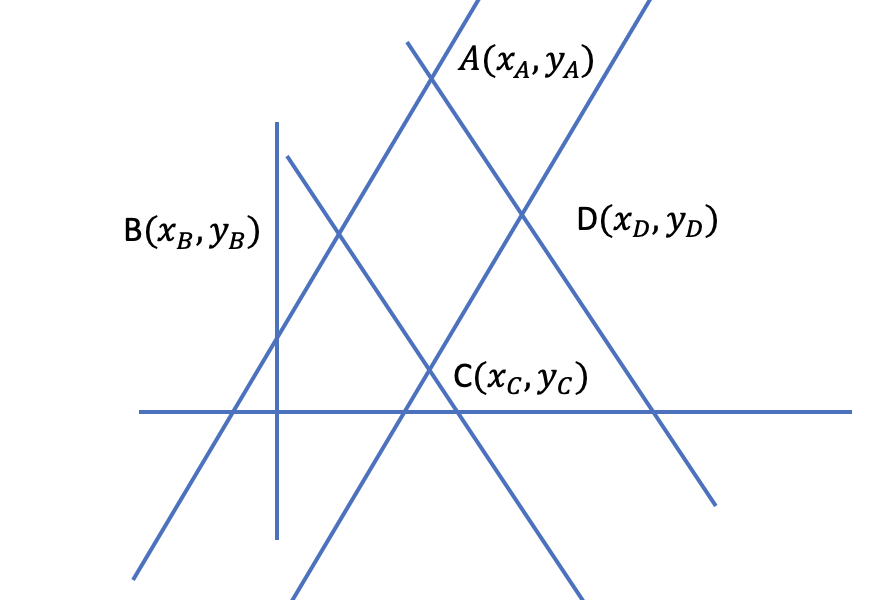
\includegraphics[width=8cm]{w2_th1}
\end{figure}
Take $c=1$ for simplicity
\[\left\{\begin{gathered}\uyy-\uxx=0\\u(x,0)=\varphi(x)\\\uy(x,0)=\psi(x)\end{gathered}\right.
\]
\[u(x,y)=f(y+x)+g(y-x)
\]
\[\varphi(x)=u(x,0)=f(x)+g(-x)
\]
\[\psi(x)=\uy(x,0)=f\p(x)+g\p(-x)
\]
\[\varphi(x)=f(x)+g(-x)~\Rightarrow~\varphi\p(x)=f\p(x)-g\p(-x)
\]
\[\dakuohao{\varphi(x)=f(x)=g(-x)}{\psi(x)=f\p(x)=g\p(x)}\Rightarrow \psi\p(x)=f\p(x)-g\p(-x)
\]
\[\frac{\varphi\p(x)+\psi(x)}{2}=f\p(x)\Rightarrow~f(x)=\frac{1}{2}\psi(x)+\frac{1}{2}\int_0^x\psi(s)\diff s+\text{const}\alpha
\]
\[\frac{-\varphi\p(x)+\psi(x)}{2}=g\p(-x)~\Rightarrow~g(-x)=\frac{1}{2}\varphi(x)-\frac{1}{2}\int_0^x\psi(s)\diff s+\text{const}\beta
\]
\[\begin{aligned}u(x,y)&=f(x+y)+g(y-x)\\&=\frac{1}{2}\varphi(x+y)+\frac{1}{2}\int_0^{x+y}\psi(s)\diff s+\alpha+\frac{1}{2}\varphi(x-y)-\frac{1}{2}\int_0^{x-y}\psi(s)\diff s+\beta\\&=\frac{1}{2}[\varphi(x+y)+\varphi(x-y)]+\frac{1}{2}\int_{x-y}^{x+y}\psi(s)\diff s+\alpha+\beta\end{aligned}
\]
\\
\[u(x,y)=\frac{1}{2}[\varphi(x+y)+\varphi(x-y)]+\frac{1}{2}\int_{x-y}^{x+y}\psi(s)\diff s
\]
\[\begin{cases}\uyy-\uxx=0\\u(x,0)=\varphi(x)\text{--initial displacement}\\\uy(x,0)=\psi(x)\text{--initial velocity}\end{cases}
\]
case(i) $\psi\equiv0$ $t=y=1$ $u(x,1)=\frac{1}{2}\varphi(x+1)+\frac{1}{2}\varphi(x-1)$
\begin{figure}[H]
\centering
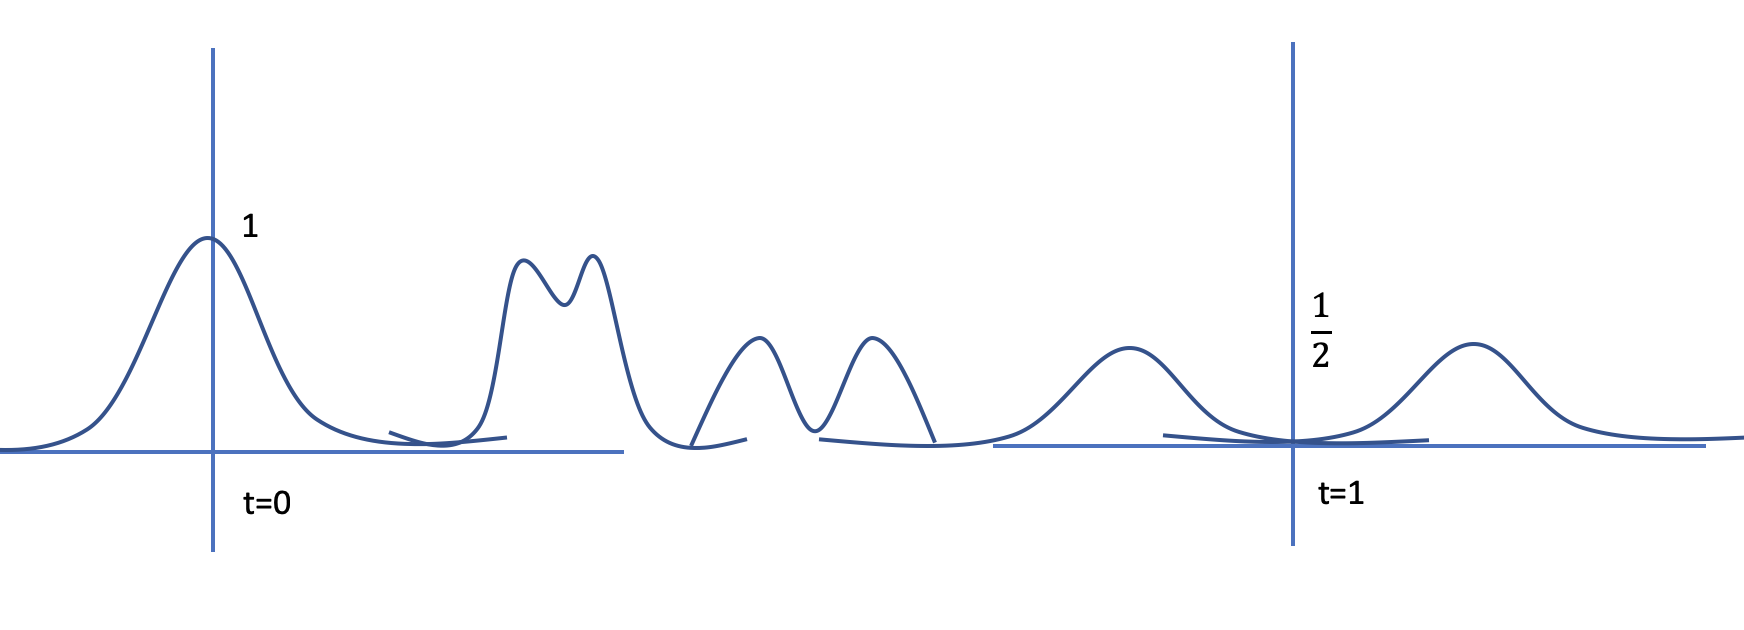
\includegraphics[width=12cm]{w2_th2}
\end{figure}
case(ii)$\psi=0$
\begin{figure}[H]
\centering
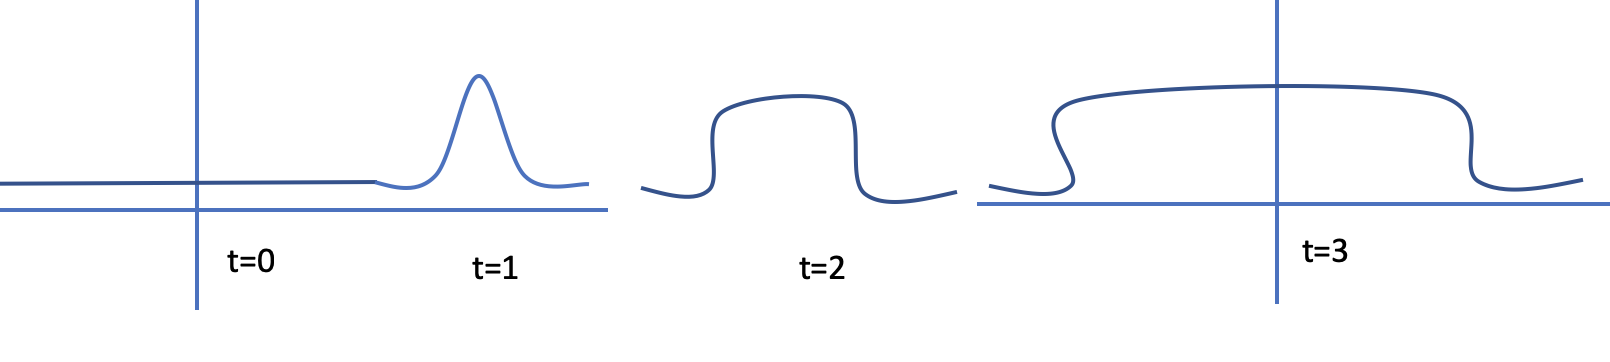
\includegraphics[width=13cm]{w2_th3}
\end{figure}
\chapter{week2}

\section{Tuesday}\index{Tuesday_lecture}
\subsection{Quasi-linear Equations}
Review: last week we have learn how to solve the following PDE and get the solution along characteristic curves.
\[\uy+c\ux=0\qquad x\ux+y\uy=u
\]
\begin{figure}[H]
\centering
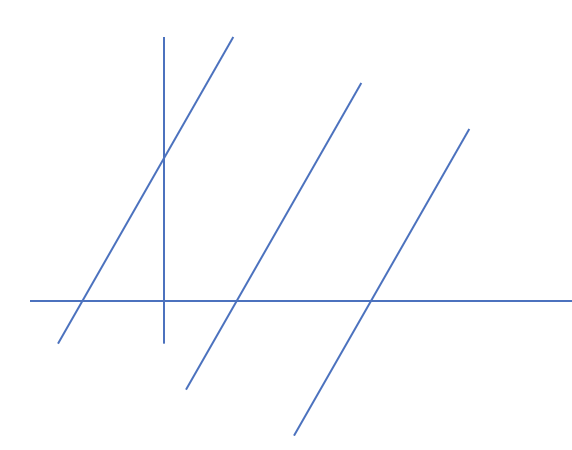
\includegraphics[width=3cm]{week2_tuesday1}
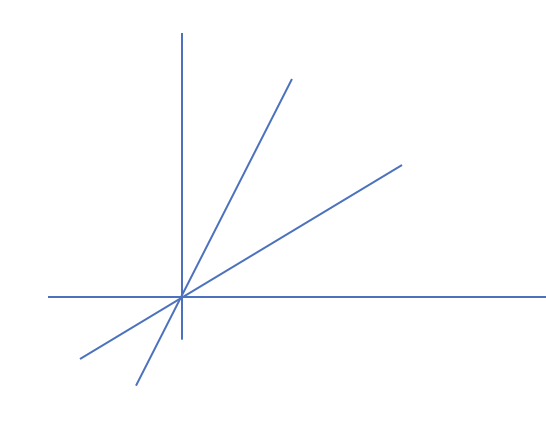
\includegraphics[width=3cm]{week2_tuesday2}
\end{figure}
\[a(x,y,u)\ux+b(x,y,u)\uy=c(x,y,u)
\]
This is what we called quasi-linear equation. At this time, I have to quote our textbook p9 since I cannot explain what professor said better than it does.
\begin{figure}[H]
\centering
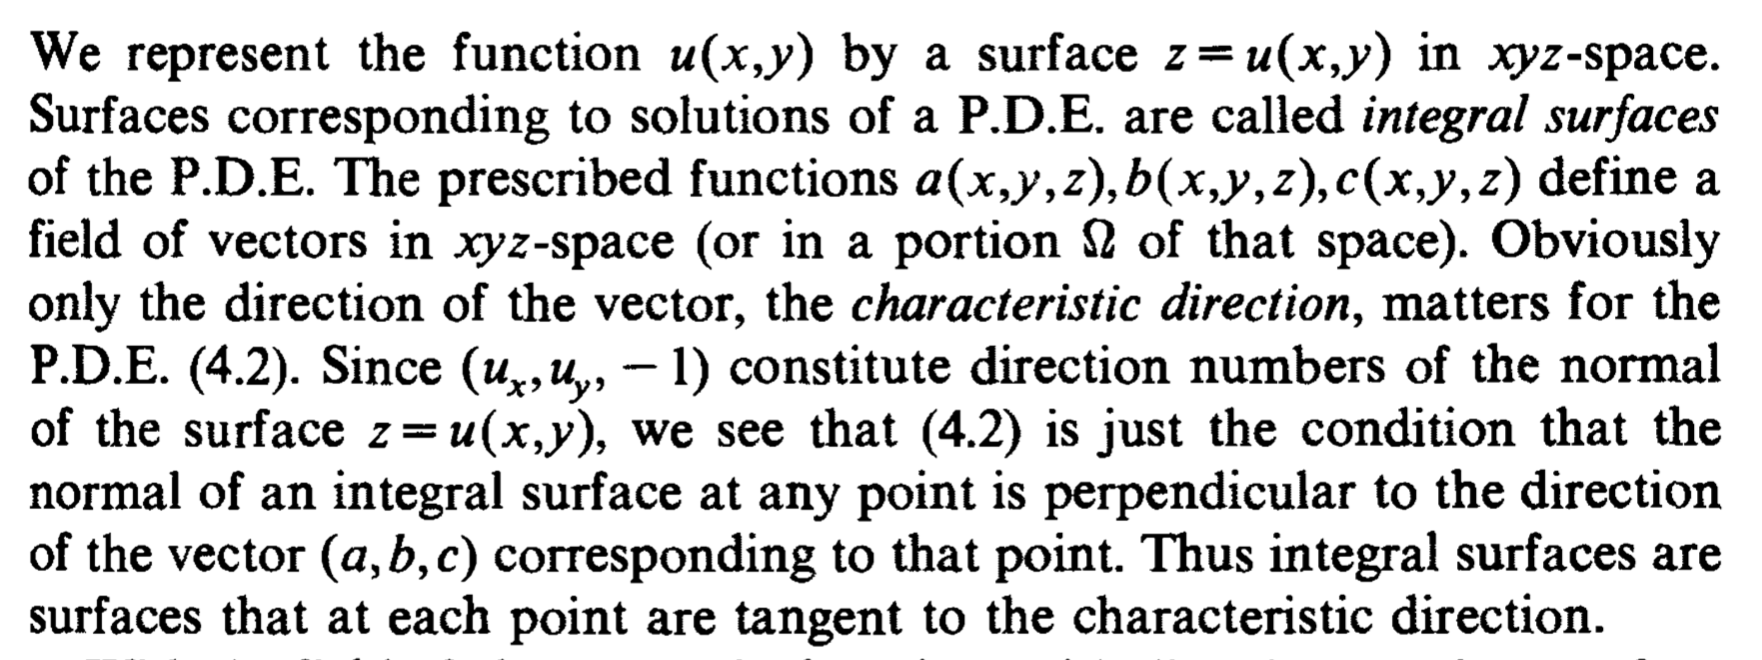
\includegraphics[width=15cm]{week2_tuesday3}
\end{figure}
\begin{figure}[H]
\centering
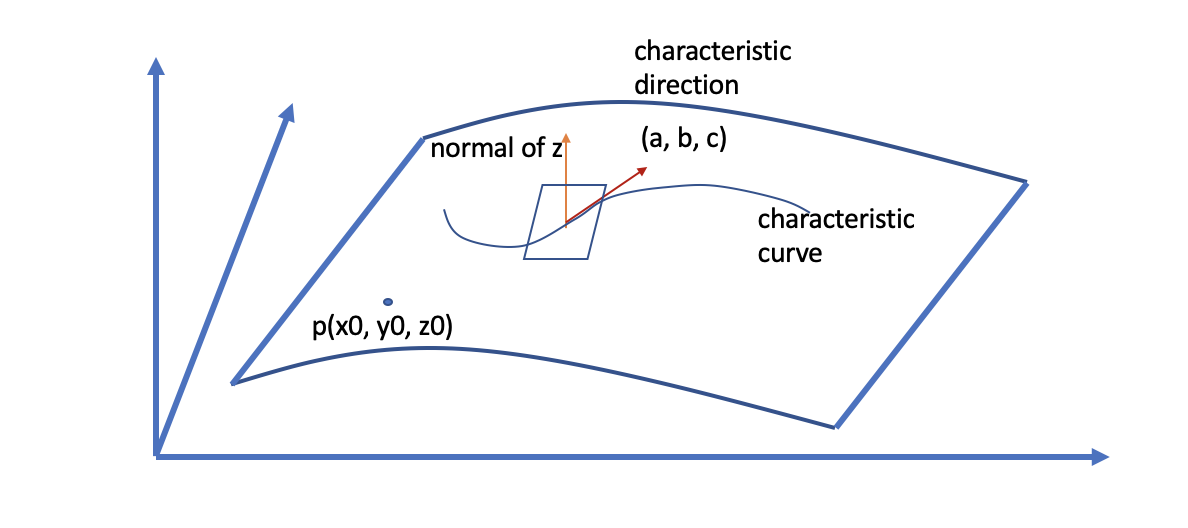
\includegraphics[width=15cm]{week2_tuesday4}
\end{figure}
Next we are going to show that the integral surface, that is the solution $u$ we want, is the union of characteristic curves.
\begin{theorem}
If a characteristic curve $\mathscr{C}$ has one point on a integral surface $z=u(x,y)$ then $\mathscr{C}$ lies entirely on the surface.

\end{theorem}
\begin{proof}
\[z_0=u(x_0,y_0)
\]
\[\left\{\begin{gathered}\deriv{x}{t}=a(x(t),y(t),u(x_0,y_0))\\\deriv{y}{t}=b(x(t),y(t),u(x_0,y_0))\\x(0)=x_0\\y(0)=y_0\end{gathered}\right.
\]
This is a system of odes, there is a solution ($x(t),y(t)$) when $t$ is around 0.\\
This gives us a curve $(x(t),y(t),u(x(t),y(t)))$ lies on the integral surface.\\
Claim: It's a characteristic curve.
\[z(t)=u(x(t),y(t))
\]
\[\deriv{z}{t}=\ux\deriv{x}{t}+\uy\deriv{y}{t}=a\ux+b\uy=c
\]



\end{proof}
\subsection{Cauchy Problem}
``We now have a simple description for the general solution $u$ of the quasilinear equation. To have a better insight into the structure of the manifold of solutions it is desirable to have a definite method of generating solutions in terms of a prescribed set $F$ of functions, called ``data''.''(John, 1982, p.11)\\
``Finding the function $u(x,y)$ for given data $x=f(s)$, $y=g(s)$, $u=h(s)$ constitutes the \text{\it Cauchy problem} for quasi-linear equation.'' (John, 1982, p.9)\\ The following $\varphi, \psi, \rho$ are $f, g, h$ correspondingly.\\
To solve the Cauchy problem, it suffices to require that $(\psi\p,\varphi\p)\&(a,b)$ are linearly independent.\\The
\[\left\{\begin{gathered}\deriv{\bar{X}}{t}=a(\bar{X},\bar{Y},Z)\\\deriv{\bar{Y}}{t}=b(\bar{X},\bar{Y},Z)\\\deriv{\bar{z}}{t}=c(\bar{X},\bar{Y},Z)\\\bar{X}(s,0)=\varphi(s)\\\bar{Y}(s,0)=\psi(s)\\\bar{Z}(s,0)=\rho(s)\end{gathered}\right.
\]
Existence and uniqueness theorem for ODE.\\
$\Rightarrow$ For every $s$, $\exists$ one solution $(\bar{X}(s,t),\bar{Y}(s,t),z(s,t))$. In order to make $u(x,y)=z(s(x,y),t(x,y))$ is the case. We need implicit function theorem which makes us able to write $s, t$ as a function of $(x,y)$
\[\begin{vmatrix}\frac{\partial{\bar{X}}}{\partial{s}}&\frac{\partial{\bar{X}}}{\partial{t}}\\\frac{\partial{\bar{Y}}}{\partial{s}}&\frac{\partial{\bar{Y}}}{\partial{t}}\end{vmatrix}=\begin{vmatrix}\varphi\p&a\\\psi\p&b\end{vmatrix}\neq0
\]
\begin{example}
\[\uy+u\ux=0, \quad u(x,0)=f(x)\]
\[\deriv{x}{t}=z,~\deriv{y}{t}=1,~\deriv{z}{t}=0
\]
$z$ is constant in $t$. $z(s, 0)=f(s)\Rightarrow z(s,t)=f(s)$.
\[\dakuohao{x(s,0)=s~\Rightarrow~x(s,t)=f(s)t+s}{y(s,0)=0~\Rightarrow~y(s,t)=t}\rightarrow ~s=x-f(s)t=x-f(s)y=x-zy
\]
\[z(s,0)=f(s)\Rightarrow z(s,t)=f(s)=f(x-zy)
\]
\[u(x,y)=f(x-uy)
\]
Characteristic curve
\[f(s_2)>f(s_3)
\]
\[\frac{1}{f(s_2)}<\frac{1}{s_3}
\]
Why it is called a ``Shock''?\\The reason is that: for same $(x,y)$ $z$ should be the same. However, from the graph we can see there are two $z$ corresponds to the same point marked by the circle. Therefore, the solution does't exist.
\begin{figure}[H]
\centering
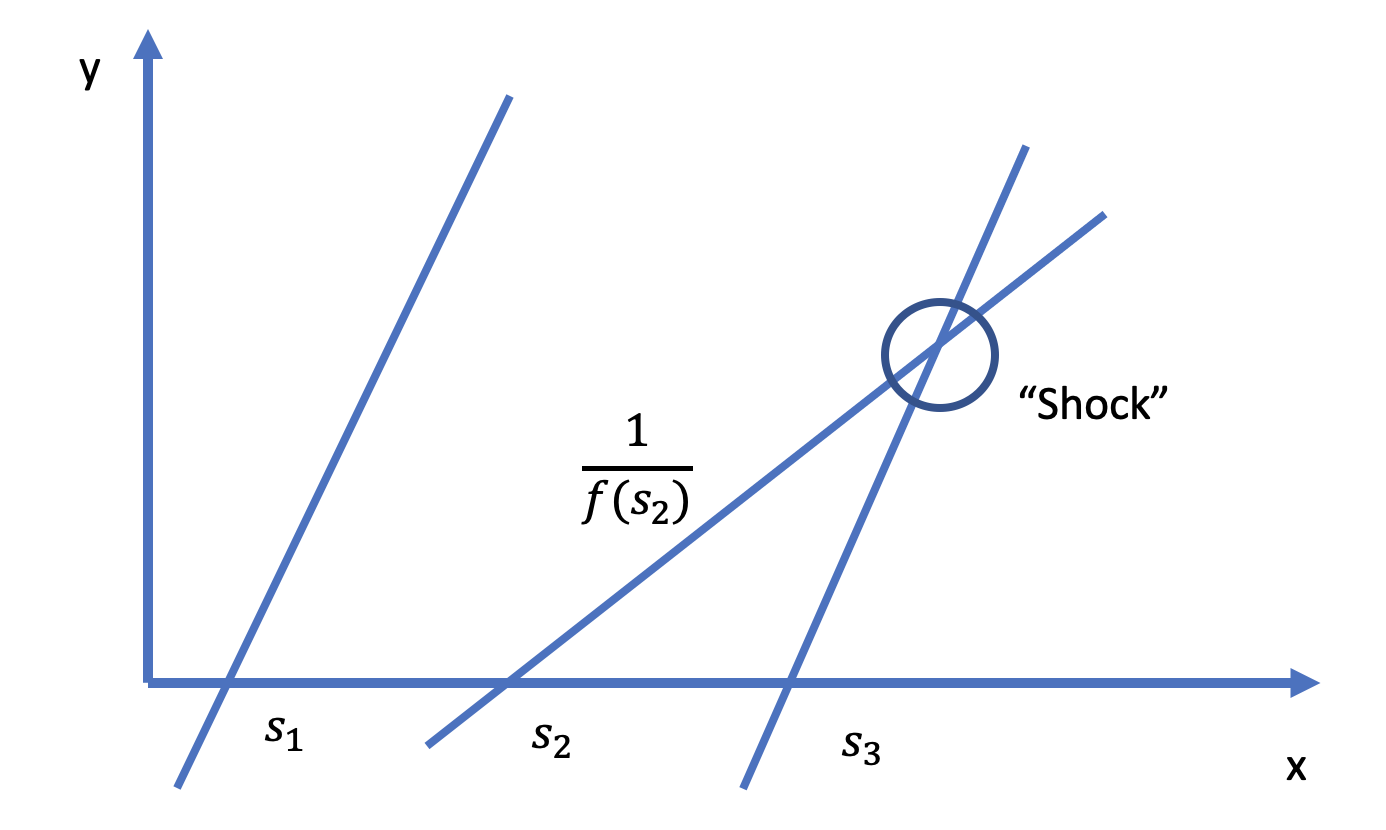
\includegraphics[width=8cm]{week2_tuesday5}
\end{figure}



\end{example}



\chapter{week3}

\section{Thursday}\index{Thursday_lecture}
\subsection{Fourier Series}
On $[-\pi,\pi]$ want to approximate $f(x)$ by $a_0+a_1\cos x+b_1\sin x+a_2\cos 2x+b_2\sin 2x+\dots+a_k\cos kx+b_k \sin kx+\dots$.\\
Want to show $\{1,\cos x,\sin x,\cos 2x,\sin 2x,\dots,\cos kx,\sin kx,\dots\}$ is a family of orthoganol functions s.t. they for a basis of continuous function space.\\
Inner product:
\[<f,g>=\int_{-\pi}^{\pi}f(x)g(x)\diff x
\]
The following is aim to show it is a orthoganol family.\\
\[<1,\cos kx>=\int_{-\pi}^\pi 1\cdot\cos kx \diff x=\frac{1}{k}\sin kx|_{-\pi}^\pi=0
\]
\[<1,\sin lx>=\int_{-\pi}^\pi 1\cdot \sin lx\diff x=-\frac{1}{L}\cos lx|_{-\pi}^\pi=0
\]
\[\begin{aligned}<\cos kx,\cos lx>&=\int_{-\pi}^\pi]\cos kx\cos lx\diff x\\
&=\frac{1}{2}\int_{-\pi}^\pi[\cos(k+l)x+\cos(k-l)x]\diff x\\
&=\frac{1}{2}\int_{-\pi}^\pi \cos(k-l)x\diff x\\
&=\begin{cases}0 \text{ if } k\neq l\\\pi \text{ if } k=l\neq0\end{cases}
\end{aligned}
\]
Next we are going to find all their coefficient.\\
Assume $f(x)=a_0+\sum_{k=1}^\infty(a_k\cos kx+b_k\sin kx)$.
\[<f,1>=\int_{-\pi}^\pi f(x)\diff x\Rightarrow a_0=\frac{1}{2\pi}\int_{-\pi}^\pi f(x)\diff x
\]
\[<a_0+\sum_{k=1}^{\infty}(a_k\cos kx+b_k\sin kx),1>=<a_0,1>+\sum_{k=1}^{\infty}<a_k\cos kx+b_k\sin kx,1>=<a_0,1>=2\pi a_0
\]
\[<f,\cos x>=<a_0,\cos x>+\sum_{k=1}^\infty[<a_k\cos kx,\cos x>+<b_k\sin kx,\cos x>]=<a_1\cos x,\cos x>=a_1\pi
\]
\[a_1=\frac{1}{\pi}\int_{-\pi}^\pi f(x)\cos x\diff x
\]
\[b_1=\frac{1}{\pi}\int_{-\pi}^\pi f(x)\sin x\diff x
\]
\[a_k=\frac{1}{\pi}\int_{-\pi}^\pi f(x)\cos kx\diff x
\]
$a_0+\sum_{k=1}^N(a_k\cos kx+b_k\sin kx)\rightarrow f(x)$ for as $N\rightarrow \infty$  $\{1,\cos x,\sin x,\cos 2x,\sin 2x,\dots,\cos kx,\sin kx,\dots\}$ form a complete basis for function space.\\
\[*\dakuohaotri{X\pp+\lambda X=0  \text{ in }(a,b)}{a_1X(a)+a_2X\p(a)=0}{\beta_1X(b)+\beta_2X\p(b)=0}
\]
$\alpha_1, \alpha_2, \beta_1, \beta_2$ are constants. $\alpha_1^2+\alpha_2^2>0,  \beta_1^2+\beta_2^2>0$
\begin{theorem}
(1) The eigenvalues of (*) form an increasing sequence $\lambda_1<\lambda_2<\lambda_3<\dots<\lambda_k<\dots\rightarrow \infty $.\\
(2)For each eigenvalue $\lambda_k$ the corresponding eigenspace is 1-dimensional. Denote eigen function by $X_k$.\\
(3) $X_k$ has exactly $k-1$ zeros in $(a,b)$.\\
(4) $\{X_1, X_2, \dots, x_k,\dots\}$ is a family of orthogonal $f(n)$ i.e. $\int_a^b x_kx_l=0$ if $k\neq l$.\\
(5)If $\varphi(x)$ is $C^2[a,b]$ then its eigen function expansion $\sum_{k=1}^\infty \varphi_k X_k$ converges to $\varphi(x)$ uniformly on $[a,b]$ when $\varphi_k=\frac{\int_a^b\varphi(x)X_k(x)\diff x}{\int_a^bX_k^2(x)\diff x}$\\
(6)If $\varphi$ is only square intergrable i.e. if $\int_a^b\varphi^2(x)\diff x<\infty$, then $\int_a^b[\varphi(x)-\sum_{k=1}^N\varphi_kX_k(x)]^2\diff x]\rightarrow 0$ as $N\rightarrow \infty$.


\end{theorem}
(1)$\dakuohao{\alpha_1=1, \alpha_2=0}{\beta_1=1, \beta_2 =0}$ Dirichlet\\
(2)$\dakuohao{\alpha_1=0,\alpha_2=1}{\beta_1=0, \beta_2=1}$ Neumann.\\
The following is going to show when two solutions of $x\pp+\lambda x=0$ are different. $x_k$ is orthorganol to $x_l$.\\
\[\dakuohao{x_k\pp+\lambda_kx_k=0}{x_l\pp+\lambda_lx_l=0}
\]
Multiply $x_l$ and $x_k$ correspondingly to two equations and then take the integral. We have
\[0=\int_a^b(x_k\pp x_l-x_l\pp x_k)+\int_a^b(\lambda_k-\lambda_l)x_kx_l=(x_k\p-x_l\p-x_l\p x_k)|_a^b+\int_a^b(\lambda_k-\lambda_l)x_kx_l
\]
\[=x_k\p(b)x_l(b)-x_l\p(b)x_k(b)-x_k\p(a)x_l(a)+x_l\p(a)x_k(a)+\int_a^b(\lambda_k-\lambda_l)x_kx_l=0
\]
\[\int_a^bx_kx_l=0
\]
Sturm-Liouville
\[\deriva{x}(p(x)\deriv{u}{x})+1(x)u=0
\]








\chapter{Week4}

\section{Tuesday}\index{Tuesday_lecture}
\subsection{Inhomogeneous Wave Equation}
\[\dakuohaotri{u_{tt}-c^2u_{xx}=f(x,t)\qquad x\in[o,L], ~t\geq0}{u(x,0)=\varphi(x), u_t(x,0)=\psi(x), ~x\in[0,L]}{u(0,t)=h(t), ~u(L,t)=k(t)}
\]
Assume $h(0)=k(0)=0$.Write 
 \[u(x,t)=\sum_{n=1}^\infty u_n(t)\sin\frac{n\pi x}{L},~u_n(t)=\frac{2}{L}\int_0^L u(x,t)\sin\frac{n\pi x}{L}\diff x\] 
\[\quad f(x,t)=\sum_{n=1}^\infty f_n(t)\sin\frac{n\pi x}{L},~f_n(t)=\frac{2}{L}\int_0^L f(x,t)\sin\frac{n\pi x}{L}\diff x\]
\[u_{tt}(x,t)=\sum_{n=1}^\infty V_n(t)\sin \frac{n\pi x}{L},\quad  V_n(t)=\frac{2}{L}\int_0^L u_{tt}(x,t)\sin \frac{n\pi x}{L}\diff x=\frac{\diff^2u_n}{\diff t}
\]
\[u_{xx}(x,t)=\sum_{n=1}^\infty w_n(t)\sin\frac{n\pi x}{L},\quad w_n(t)=\frac{2}{L}\int_0^L u_{xx}(x,t)\sin \frac{n\pi x}{L}\diff x
\]
\[\begin{aligned}w_n(t)&=\frac{2}{L}\int_0^L \uxx(x,t)\sin\frac{n\pi x}{L}\diff x\\
&=\frac{2}{L}[\ux\sin\frac{n\pi x}{L}|_0^L-\frac{n\pi}{L}\int_0^L\ux\cos \frac{n\pi x}{L}\diff x]\\
&=-\frac{2n\pi}{L^2}[n\cos\frac{n\pi x}{L}|_0^L+\frac{n\pi}{L}\int_0^Lu\sin\frac{n\pi x}{L}\diff x]\\
&=-\frac{2n\pi}{L^2}[u(L,t)(-1)^n-u(0,t)+\frac{n\pi}{L}\int_0^Lu\sin\frac{n\pi x}{L}\diff x]\\
&=-\frac{2n\pi}{L^2}[(-1)^nk(t)-h(t)+\frac{n\pi}{2}u_n(t)]\\
&=\frac{2n\pi}{L^2}[h(t)-(-1)^nk(t)]-(\frac{n\pi}{L})^2u_n(t)
\end{aligned}
\]
\[v_n(t)-c^2w_n(t)=\frac{2}{L}\int_0^L(u_{tt}-c^2\uxx)\sin\frac{n\pi x}{L}\diff x=\frac{2}{L}\int_0^Lf(x,t)\sin\frac{n\pi x}{L}\diff x=f_n(t)
\]
\[\frac{\diff^2u_n}{\diff t^2}+c^2\lambda_nu_n(t)-\frac{2n\pi}{L^2}[h(t)-(-1)^nk(t)]c^2=f_n(t),~n\geq1
\]
Solve this ODE of $u_n$, we get the solution.\\
%\[\dakuohao{u_tt-c^2\uxx=f(x,t)}{u(0,t)=u(L,t)=0}
%\]
\[\dakuohao{u_{tt}-c^2\uxx=f(x,t)}{u(0,t=u(L,t)=0}
\]
To solve
\[\dakuohao{U_{tt}-c^2U_{xx}=g(x,t)}{U(0,L)=h(t), U(L,t)=k(t)}
\]
Set $\rho(x,t)=\frac{(L-x)}{L}h(t)+\frac{x}{L}k(t)~\Rightarrow~ \rho(0,t)=h(t),~\rho(L,t)=k(t)$
\[u(x,t)=U(x,t)-\rho(x,t)
\]
\[u_{tt}-c^2\uxx=U_{tt}-c^2U_{xx}-\rho_{tt}+c^2\rho_{xx}=g(x,t)-\frac{L-x}{L}h_{tt}-\frac{x}{L}k_{tt}=f(x,t)
\]
Set $U(x,t)=u(x,t)+\frac{L-x}{L}h(t)+\frac{x}{L}k(t)$.


%%%%%%%%%%%%%%%%%%
To solve the given inhomogeneous problem
\[\dakuohao{U_{tt}-c^2U_{xx}=g(x,t)}{U(0,L)=h(t), U(L,t)=k(t)}
\]
Set $f(x,t)=g(x,t)-\frac{L-x}{L}h_{tt}(t)-\frac{x}{L}k_{tt}(t)$ and we know the solution for $\dakuohao{u_tt-c^\uxx=f(x,t)}{u(0,t)=0,~u(L,t)=0}$ Then $U(x,t)=u(x,t)+\frac{L-x}{L}h(t)+\frac{x}{L}k(t)$ solves.
%%%%%%%%%%%%
Solve $\dakuohao{v_{tt}-c^2v_{xx}=0}{v(x,0)=\varphi(x), v_t(x,0)=\psi(x)}\Rightarrow U+v$\\

\[\dakuohaotri{u_{tt}-c^2\uxx=f(x,t)\quad x\in\mathbb{R},t\geq0}{u(x,0)=\varphi(x)}{u_r(x,0)=\psi(x)}
\]
\[u(x,t)=\frac{1}{2}(\varphi(x+ct)+\varphi(x-ct))+\frac{1}{2c}\int_{x-ct}^{x+ct}\psi(y)\diff y+\frac{1}{2c}\int\int_Df(y,s)\diff y\diff s
\]
Duhamel's Principle
\[\dakuohaotri{\frac{\diff^2v}{\diff t^2}+A^2v=f(t)}{v(0)=a}{v\p(0)=b}
\]
Let $S(t)=\frac{1}{A}\sin At~\Rightarrow ~v(t)=S\p(t)a+S(t)b+\int_0^tS(t-s)f(s)\diff s$\\
Pluge $S$ in the system of equations. We get the solution. (Remind what we do in ODE with variation of parameter. This two method is the same in essence. In addition, what we do in PDE is similiar.)
















\chapter{week3}

\section{Thursday}\index{Thursday_lecture}
\subsection{Fourier Series}
On $[-\pi,\pi]$ want to approximate $f(x)$ by $a_0+a_1\cos x+b_1\sin x+a_2\cos 2x+b_2\sin 2x+\dots+a_k\cos kx+b_k \sin kx+\dots$.\\
Want to show $\{1,\cos x,\sin x,\cos 2x,\sin 2x,\dots,\cos kx,\sin kx,\dots\}$ is a family of orthoganol functions s.t. they for a basis of continuous function space.\\
Inner product:
\[<f,g>=\int_{-\pi}^{\pi}f(x)g(x)\diff x
\]
The following is aim to show it is a orthoganol family.\\
\[<1,\cos kx>=\int_{-\pi}^\pi 1\cdot\cos kx \diff x=\frac{1}{k}\sin kx|_{-\pi}^\pi=0
\]
\[<1,\sin lx>=\int_{-\pi}^\pi 1\cdot \sin lx\diff x=-\frac{1}{L}\cos lx|_{-\pi}^\pi=0
\]
\[\begin{aligned}<\cos kx,\cos lx>&=\int_{-\pi}^\pi]\cos kx\cos lx\diff x\\
&=\frac{1}{2}\int_{-\pi}^\pi[\cos(k+l)x+\cos(k-l)x]\diff x\\
&=\frac{1}{2}\int_{-\pi}^\pi \cos(k-l)x\diff x\\
&=\begin{cases}0 \text{ if } k\neq l\\\pi \text{ if } k=l\neq0\end{cases}
\end{aligned}
\]
Next we are going to find all their coefficient.\\
Assume $f(x)=a_0+\sum_{k=1}^\infty(a_k\cos kx+b_k\sin kx)$.
\[<f,1>=\int_{-\pi}^\pi f(x)\diff x\Rightarrow a_0=\frac{1}{2\pi}\int_{-\pi}^\pi f(x)\diff x
\]
\[<a_0+\sum_{k=1}^{\infty}(a_k\cos kx+b_k\sin kx),1>=<a_0,1>+\sum_{k=1}^{\infty}<a_k\cos kx+b_k\sin kx,1>=<a_0,1>=2\pi a_0
\]
\[<f,\cos x>=<a_0,\cos x>+\sum_{k=1}^\infty[<a_k\cos kx,\cos x>+<b_k\sin kx,\cos x>]=<a_1\cos x,\cos x>=a_1\pi
\]
\[a_1=\frac{1}{\pi}\int_{-\pi}^\pi f(x)\cos x\diff x
\]
\[b_1=\frac{1}{\pi}\int_{-\pi}^\pi f(x)\sin x\diff x
\]
\[a_k=\frac{1}{\pi}\int_{-\pi}^\pi f(x)\cos kx\diff x
\]
$a_0+\sum_{k=1}^N(a_k\cos kx+b_k\sin kx)\rightarrow f(x)$ for as $N\rightarrow \infty$  $\{1,\cos x,\sin x,\cos 2x,\sin 2x,\dots,\cos kx,\sin kx,\dots\}$ form a complete basis for function space.\\
\[*\dakuohaotri{X\pp+\lambda X=0  \text{ in }(a,b)}{a_1X(a)+a_2X\p(a)=0}{\beta_1X(b)+\beta_2X\p(b)=0}
\]
$\alpha_1, \alpha_2, \beta_1, \beta_2$ are constants. $\alpha_1^2+\alpha_2^2>0,  \beta_1^2+\beta_2^2>0$
\begin{theorem}
(1) The eigenvalues of (*) form an increasing sequence $\lambda_1<\lambda_2<\lambda_3<\dots<\lambda_k<\dots\rightarrow \infty $.\\
(2)For each eigenvalue $\lambda_k$ the corresponding eigenspace is 1-dimensional. Denote eigen function by $X_k$.\\
(3) $X_k$ has exactly $k-1$ zeros in $(a,b)$.\\
(4) $\{X_1, X_2, \dots, x_k,\dots\}$ is a family of orthogonal $f(n)$ i.e. $\int_a^b x_kx_l=0$ if $k\neq l$.\\
(5)If $\varphi(x)$ is $C^2[a,b]$ then its eigen function expansion $\sum_{k=1}^\infty \varphi_k X_k$ converges to $\varphi(x)$ uniformly on $[a,b]$ when $\varphi_k=\frac{\int_a^b\varphi(x)X_k(x)\diff x}{\int_a^bX_k^2(x)\diff x}$\\
(6)If $\varphi$ is only square intergrable i.e. if $\int_a^b\varphi^2(x)\diff x<\infty$, then $\int_a^b[\varphi(x)-\sum_{k=1}^N\varphi_kX_k(x)]^2\diff x]\rightarrow 0$ as $N\rightarrow \infty$.


\end{theorem}
(1)$\dakuohao{\alpha_1=1, \alpha_2=0}{\beta_1=1, \beta_2 =0}$ Dirichlet\\
(2)$\dakuohao{\alpha_1=0,\alpha_2=1}{\beta_1=0, \beta_2=1}$ Neumann.\\
The following is going to show when two solutions of $x\pp+\lambda x=0$ are different. $x_k$ is orthorganol to $x_l$.\\
\[\dakuohao{x_k\pp+\lambda_kx_k=0}{x_l\pp+\lambda_lx_l=0}
\]
Multiply $x_l$ and $x_k$ correspondingly to two equations and then take the integral. We have
\[0=\int_a^b(x_k\pp x_l-x_l\pp x_k)+\int_a^b(\lambda_k-\lambda_l)x_kx_l=(x_k\p-x_l\p-x_l\p x_k)|_a^b+\int_a^b(\lambda_k-\lambda_l)x_kx_l
\]
\[=x_k\p(b)x_l(b)-x_l\p(b)x_k(b)-x_k\p(a)x_l(a)+x_l\p(a)x_k(a)+\int_a^b(\lambda_k-\lambda_l)x_kx_l=0
\]
\[\int_a^bx_kx_l=0
\]
Sturm-Liouville
\[\deriva{x}(p(x)\deriv{u}{x})+1(x)u=0
\]







\chapter{week2}

\section{Tuesday}\index{Tuesday_lecture}
\subsection{Quasi-linear Equations}
Review: last week we have learn how to solve the following PDE and get the solution along characteristic curves.
\[\uy+c\ux=0\qquad x\ux+y\uy=u
\]
\begin{figure}[H]
\centering
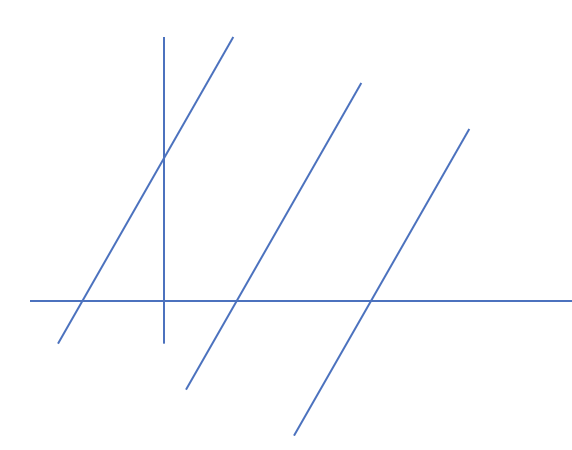
\includegraphics[width=3cm]{week2_tuesday1}
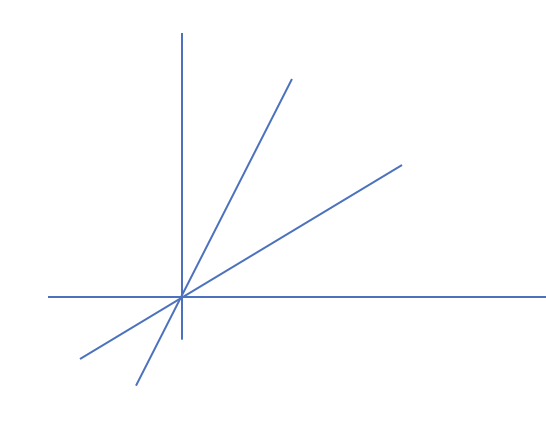
\includegraphics[width=3cm]{week2_tuesday2}
\end{figure}
\[a(x,y,u)\ux+b(x,y,u)\uy=c(x,y,u)
\]
This is what we called quasi-linear equation. At this time, I have to quote our textbook p9 since I cannot explain what professor said better than it does.
\begin{figure}[H]
\centering
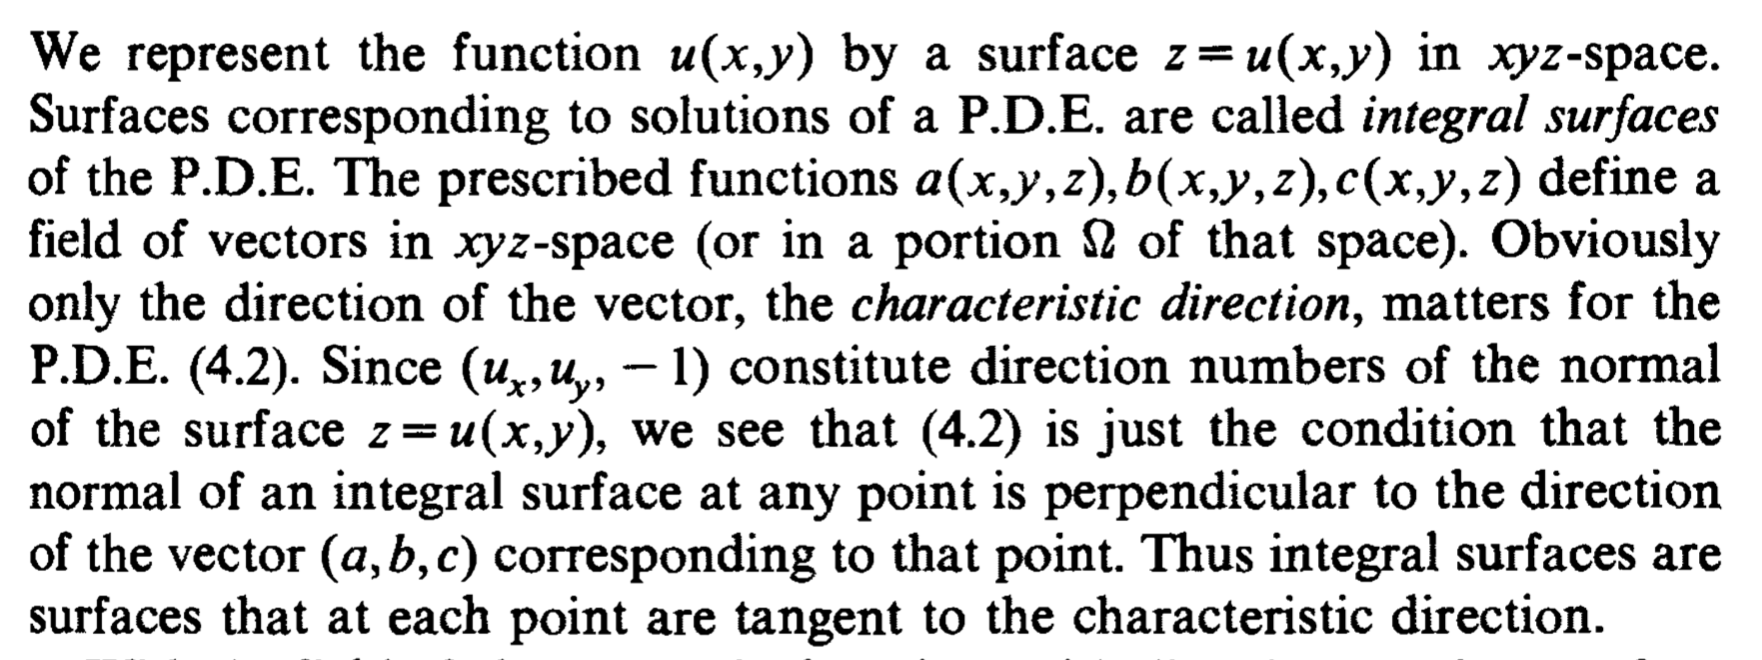
\includegraphics[width=15cm]{week2_tuesday3}
\end{figure}
\begin{figure}[H]
\centering
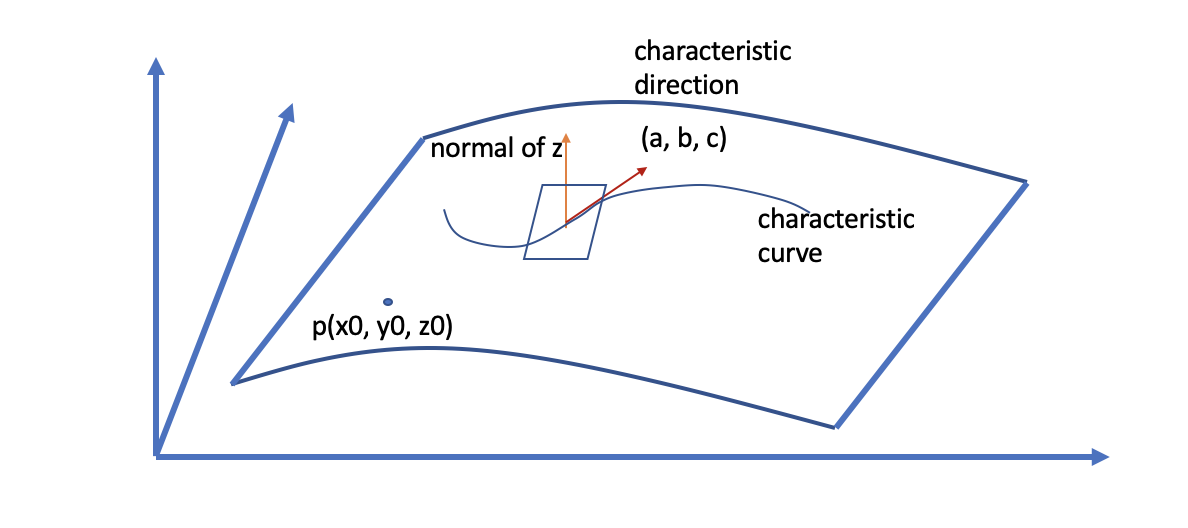
\includegraphics[width=15cm]{week2_tuesday4}
\end{figure}
Next we are going to show that the integral surface, that is the solution $u$ we want, is the union of characteristic curves.
\begin{theorem}
If a characteristic curve $\mathscr{C}$ has one point on a integral surface $z=u(x,y)$ then $\mathscr{C}$ lies entirely on the surface.

\end{theorem}
\begin{proof}
\[z_0=u(x_0,y_0)
\]
\[\left\{\begin{gathered}\deriv{x}{t}=a(x(t),y(t),u(x_0,y_0))\\\deriv{y}{t}=b(x(t),y(t),u(x_0,y_0))\\x(0)=x_0\\y(0)=y_0\end{gathered}\right.
\]
This is a system of odes, there is a solution ($x(t),y(t)$) when $t$ is around 0.\\
This gives us a curve $(x(t),y(t),u(x(t),y(t)))$ lies on the integral surface.\\
Claim: It's a characteristic curve.
\[z(t)=u(x(t),y(t))
\]
\[\deriv{z}{t}=\ux\deriv{x}{t}+\uy\deriv{y}{t}=a\ux+b\uy=c
\]



\end{proof}
\subsection{Cauchy Problem}
``We now have a simple description for the general solution $u$ of the quasilinear equation. To have a better insight into the structure of the manifold of solutions it is desirable to have a definite method of generating solutions in terms of a prescribed set $F$ of functions, called ``data''.''(John, 1982, p.11)\\
``Finding the function $u(x,y)$ for given data $x=f(s)$, $y=g(s)$, $u=h(s)$ constitutes the \text{\it Cauchy problem} for quasi-linear equation.'' (John, 1982, p.9)\\ The following $\varphi, \psi, \rho$ are $f, g, h$ correspondingly.\\
To solve the Cauchy problem, it suffices to require that $(\psi\p,\varphi\p)\&(a,b)$ are linearly independent.\\The
\[\left\{\begin{gathered}\deriv{\bar{X}}{t}=a(\bar{X},\bar{Y},Z)\\\deriv{\bar{Y}}{t}=b(\bar{X},\bar{Y},Z)\\\deriv{\bar{z}}{t}=c(\bar{X},\bar{Y},Z)\\\bar{X}(s,0)=\varphi(s)\\\bar{Y}(s,0)=\psi(s)\\\bar{Z}(s,0)=\rho(s)\end{gathered}\right.
\]
Existence and uniqueness theorem for ODE.\\
$\Rightarrow$ For every $s$, $\exists$ one solution $(\bar{X}(s,t),\bar{Y}(s,t),z(s,t))$. In order to make $u(x,y)=z(s(x,y),t(x,y))$ is the case. We need implicit function theorem which makes us able to write $s, t$ as a function of $(x,y)$
\[\begin{vmatrix}\frac{\partial{\bar{X}}}{\partial{s}}&\frac{\partial{\bar{X}}}{\partial{t}}\\\frac{\partial{\bar{Y}}}{\partial{s}}&\frac{\partial{\bar{Y}}}{\partial{t}}\end{vmatrix}=\begin{vmatrix}\varphi\p&a\\\psi\p&b\end{vmatrix}\neq0
\]
\begin{example}
\[\uy+u\ux=0, \quad u(x,0)=f(x)\]
\[\deriv{x}{t}=z,~\deriv{y}{t}=1,~\deriv{z}{t}=0
\]
$z$ is constant in $t$. $z(s, 0)=f(s)\Rightarrow z(s,t)=f(s)$.
\[\dakuohao{x(s,0)=s~\Rightarrow~x(s,t)=f(s)t+s}{y(s,0)=0~\Rightarrow~y(s,t)=t}\rightarrow ~s=x-f(s)t=x-f(s)y=x-zy
\]
\[z(s,0)=f(s)\Rightarrow z(s,t)=f(s)=f(x-zy)
\]
\[u(x,y)=f(x-uy)
\]
Characteristic curve
\[f(s_2)>f(s_3)
\]
\[\frac{1}{f(s_2)}<\frac{1}{s_3}
\]
Why it is called a ``Shock''?\\The reason is that: for same $(x,y)$ $z$ should be the same. However, from the graph we can see there are two $z$ corresponds to the same point marked by the circle. Therefore, the solution does't exist.
\begin{figure}[H]
\centering
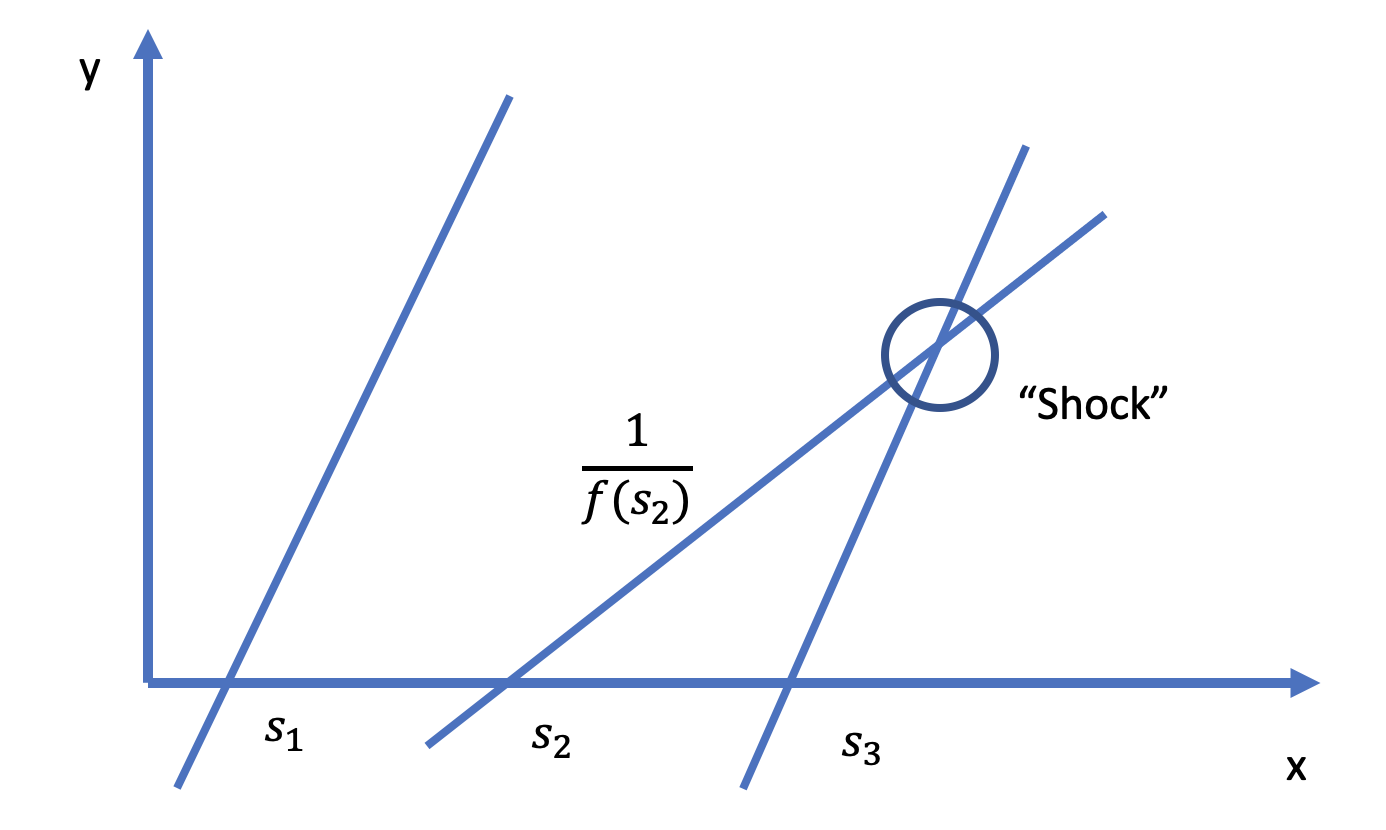
\includegraphics[width=8cm]{week2_tuesday5}
\end{figure}



\end{example}


\section{Thursday}\index{Thursday_lecture}
\subsection{Fourier Transformation}
\[f \in C_0^\infty(\mathbb{R}), f(x)
\]
\[\hat{f}(\xi)=\frac{1}{\sqrt{2\pi}}\int_{-\infty}^\infty e^{-ix\xi}f(x)\diff x
\]
Fourier transform of $f$.\\
\[e^{i\theta}=\cos\theta+i\sin\theta
\]
Use fourier transform to change PDE to ODE.
\[\begin{aligned}\widehat{f}\p(\xi)&=\frac{1}{\sqrt{2\pi}}\int_{-\infty}^\infty e^{-ix\xi}f\p(x)\diff x\\
&=-\frac{1}{\sqrt{2\pi}}\int_{-\infty}^\infty(\deriva{x}e^{-ix\xi})f(x)\diff x\\
&=i\xi\frac{1}{\sqrt{2\pi}}\int_{-\infty}^\infty e^{-ix\xi}f(x)\diff x=i\xi \hat{f}(\xi)
\end{aligned}
\]

\[\ut=\uxx,\quad u(x,0)=\varphi(x) on \mathbb{R}
\]
\[\hat{\ut}=\hat{\uxx}=i\xi\hat{\ux}=(i\xi)^2\hat{u}=-\xi^2\hat{u}
\]
\[\hat{\ut}(\xi,t)=-\xi^2\hat{u}(\xi,t)
\]
\[\hat{u}(\xi,t)=C(\xi)e^{-\xi^2t}
\]
\[\hat{u}(\xi,0)=\hat{\varphi}(\xi)=C(\xi)
\]
\[\hat{u}(\xi,t)=\hat{\varphi}(\xi)e^{-\xi^2t}
\]
Inverse Fourier Transform
\[f(x)=\frac{1}{\sqrt{2\pi}}\int_{-\infty}^\infty e^{ix\xi}\hat{f}(\xi)\diff \xi
\]
\[u(x)=\frac{1}{\sqrt{2\pi}}\int_{-\infty}^\infty e^{ix\xi}\hat{\varphi}(\xi)e^{-\xi^2 t}\diff \xi=\frac{1}{2\pi}\int_{-\infty}^\infty(\int_{-\infty}^\infty e^{ix\xi-iy\xi-\xi^2t}\diff \xi)\varphi(y)\diff y
\]
where $\hat{\varphi}(\xi)=\frac{1}{\sqrt{2\pi}}\int_{-\infty}^\infty e^{-iy\xi}\varphi(y)\diff y$
\[K(x,y,t)=\frac{1}{2\pi}\int_{-\infty}^\infty e^{i(x-y)\xi-\xi^2t}\diff \xi=\frac{1}{2\pi}\int_{-\infty}^\infty e^{-t(\xi-\frac{i(x-y)}{2t})^2}e^{-\frac{(x-y)^2}{4t}}\diff \xi
\]
where $i(x-y)\xi-\xi^2t=-t[\xi^2-i\frac{x-y}{t}\xi+(\frac{i(x-y)}{2t})^2)]-\frac{(x-y)^2}{4t}$. We have
\[\begin{aligned}K(x,y,t)&=\frac{1}{2\pi}e^{-\frac{(x-y)^2}{4t}}\int_{-\infty}^\infty e^{-t[\xi-i\frac{(x-y)}{2t}]^2}\diff \xi\quad t>0\\
&=\frac{1}{2\pi}e^{-\frac{(x-y)^2}{4t}}\int_{-\infty}^\infty e^{-[\sqrt{t}\xi-\frac{i(x-y)}{2\sqrt{t}}]^2}\diff \xi
\end{aligned}
\]
Let $\eta=\sqrt{t}\xi-\frac{i(x-y)}{2\sqrt{t}}$ and $\diff \eta=\sqrt{t}\diff \xi$. Above is equal to \[\frac{1}{2\pi}e^{-\frac{(x-y)^2}{4t}}(\int_{-\infty}^\infty e^{-\eta^2}\diff \eta)\frac{1}{\sqrt{t}}=\frac{1}{\sqrt{4\pi t}}e^{-\frac{(x-y)^2}{4t}} 
\]
\[K(x,y,t)=\frac{1}{\sqrt{4\pi t}}e^{-\frac{(x-y)^2}{4t}} \text{  Heat Kernel}
\]
\[u(x,t)=\frac{1}{\sqrt{4\pi t}}\int_{-\infty}^\infty e^{-\frac{(x-y)^2}{4t}}\varphi(y)\diff y=\int_{-\infty}^\infty K(x,y,t)\varphi(y)\diff y
\]
\begin{theorem}
Let $\varphi$ be a bounded continuous function on $\mathbb{R}$. Then 
\[u(x,t)=\int_{-\infty}^\infty K(x,y,t)\varphi(y)\diff y=\frac{1}{\sqrt{4\pi t}}\int_{-\infty}^\infty e^{-\frac{(x-y)^2}{4t}}\varphi(y)\diff y, ~t>0\] 
is a solution for $\ut=\uxx$ with $\lim_{x\rightarrow x_0~ t\rightarrow0}u(x,t)=\varphi(x_0)$ for any $x_o\in\mathbb{R}$. 

\end{theorem}
\begin{proof}
Basic properties of $K:t>0$\\
(1) $K$ is $C^\infty$ $\forall x,y \in \mathbb{R}, t>0$\\
(2) $(K_t-K_{xx})(x,y,t)=0, ~t>o$\\
(3) $K(x,y,t)>0$\\
(4) $\int_{-\infty}^\infty K(x,y,t)\diff y=1~\forall x\in\mathbb{R}, t>0$\\
(5) For any $\epsilon>0$, $\int K(x,y,t)\diff y\rightarrow0$ uniformly in x, as $t\rightarrow0~|x-y|>\epsilon$ 
\end{proof}
\begin{remark}
1.$u\in C^\infty$ as soon as $t$ becomes positive.\\
2. Speed of propogation of `` heat'' transfer is $\infty$.\\
3. $\inf_{x\in\mathbb{R}}\varphi(x)\leq u(x,t)\leq \sup_{x\in\mathbb{R}}\varphi(x)$ (Max principle. )\\
4. Soltion is NOT unique.

\end{remark}

List of Properties:function $\rightarrow$ after transformation
\begin{itemize}
\item $f\p(x)$ $\rightarrow$  $i\xi\hat{f}(\xi)$\\
\item $xf(x)$  $\rightarrow$  $i\hat{f}\p(\xi)$\\
\item $f(x-a)$  $\rightarrow$  $e^{-ia\xi}\hat{f}(\xi)$\\
\item $e^{iax}$  $\rightarrow$  $ \hat{f}(\xi-a)$\\
\item $f(ax)$  $\rightarrow$  $\frac{1}{|a|}\hat{f}(\frac{\xi}{a})$, $(a\neq0)$
\end{itemize}
\begin{definition}
A distribution is a linear functional $f[\phi]$ defined for all $\phi\in C_0^\infty(\Omega)$, which is continuous in the following sense:\\
Let $\{\phi_k\}$ a sequence of functions in $C_0^\infty(\Omega)$ s.t. \\
(i) Support $\phi_l\subset K<< \Omega, \forall l$ (K: independent of l)\\
(ii) $D^\alpha\phi_l\rightarrow 0$ uniformly in $x\in \Omega$ for each $\alpha$.\\
Then $\lim_{l\rightarrow\infty}f[\phi_l]=0$
\end{definition}
\begin{remark}
Support is a mathematical concept.
\end{remark}
\begin{example}
1 $f$ is a functional. $f[\phi]=\int_\Omega f\phi\quad \phi\in C_0^\infty(\Omega)$\\
2. Dirac $\delta$-function, x is fixed in $\Omega$
\[\delta_x[\phi]=\int_\Omega\delta_x\phi=\phi(x)
\]
\end{example}
List: function $\rightarrow$ Fourier transformation\\
$\delta(x)\rightarrow \frac{1}{2\pi}$\\
$e^{-a|x|}\rightarrow\frac{1}{\sqrt{2\pi}}\frac{2a}{a^2+\xi^2}~a>0$\\
$1\rightarrow\sqrt{2\pi}\delta(\xi)$\\
$e^{-\frac{x^2}{2}}\rightarrow e^{-\frac{\xi^2}{2}}$\\
$H(a-|x|)\rightarrow \frac{1}{2\pi}\frac{2}{\xi}\sin(a\xi), a>0$
\begin{remark}
$\hat{f}\p$ and $\widehat{f\p}$ are different. Be careful.

\end{remark}


\backmatter


\end{document}
